\chapter{Benchmark}
L'obiettivo dell'esercizio è quello di confrontare due sistemi con lo stesso sistema operativi, ma processori differenti, utilizzando il benchmark \textit{Nbody}. Esso simula l'evoluzione di N corpi celesti, sotto l'influenza della forza di gravità ed è molto utile per confrontare le prestazioni tra i due sistemi, dato che stressa:
\begin{itemize}
	\item \textbf{CPU}
	\item \textbf{Sottosistemi Floating-Point}
	\item \textbf{Chiamate ricorsive}
\end{itemize}
La complessità dell'algoritmo che lo implementa è un \textit{O($n^2$)}.

\section{Sistemi}
Il confronto avviene tramite due macchine virtuali, su architetture diverse. Ogni macchina virtuale però è stata dotata delle stesse caratteristiche e prestazioni, in modo da ridurre il più possibile l'eterogeneità tra i due sistemi fisici. L'unico fattore su cui non si può agire è il processore. 
\\Per rendere il confronto quanto il più possibile affidabile è stata usata anche la stessa versione dell'hypervisor (in questo caso VirtualBox).
\begin{table}[H]
	\begin{center}
		\begin{tabularx}{0.49\textwidth}{|c|X|}
			\hline
			\multicolumn{2}{|c|}{\textbf{Sistema 1}} \\
			\hline
			\textit{CPU} & Intel Core i7-7500U 7th Generation - 2.70 GHz \\
			\hline
			\textit{Memoria Centrale} & 2 GB \\
			\hline
			\textit{Hard-Disk} & 25 GB - SSD \\
			\hline
			\textit{Memoria Video} & 16 MB \\
			\hline
			\textit{OS} & Xubuntu 20.04 LTS - 64bit \\
			\hline
		\end{tabularx}
		\begin{tabularx}{0.49\textwidth}{|c|X|}
			\hline
			\multicolumn{2}{|c|}{\textbf{Sistema 2}} \\
			\hline
			\textit{CPU} & Intel Core i5-5700U 5th Generation - 2.20 GHz\\
			\hline
			\textit{Memoria Centrale} & 2 GB \\
			\hline
			\textit{Hard-Disk} & 25 GB - SSD \\
			\hline
			\textit{Memoria Video} & 16 MB \\
			\hline
			\textit{OS} & Xubuntu 20.04 LTS - 64bit \\
			\hline
		\end{tabularx}
	\end{center}
\end{table}
Ogni macchina virtuale è stata dotata di 2 processori.
\section{Test e Risultati}
Su entrambi i sistemi è stato avviato lo script \textit{launch\_nbody.sh}, con i seguenti parametri di input:
\begin{minted}[framesep = 1mm,
	fontsize = \footnotesize,
	breaklines,
	]{PYTHON}
	./launch_nbody.sh -r 25 -n N
\end{minted}
Esso non fa altro che lanciare l'eseguibile \textit{nbodySim} per un numero di ripetizioni impostato a 25. 
\textit{nbodySim} esegue sul sistema l'algoritmo che implementa il benchmark in questione.
\\
Lo script è stato eseguito facendo variare di volta in volta N:
\begin{equation*}
	N = \begin{bmatrix}
		10 & 100 & 500 & 1.000 & 5.000 & 10.000 & 50.000 & 100.000 & 500.000 & 1.000.000
	\end{bmatrix}
\end{equation*}
L'output fornito da \textit{nbodySim} consiste nel tempo d'esecuzione (in microsecondi) impiegato dal sistema per eseguire l'algoritmo. 
Dunque per ogni valore di N sono state effettuate 25 misurazioni, ciascuna delle quali è stata collezionata in un file \textit{.csv} per poter poi essere processata attraverso il seguente script MATLAB
\begin{minted}[framesep = 1mm,
	fontsize = \footnotesize,
	breaklines,
	]{MATLAB}
%% Read 
N = [10 100 500 1000 5000 10000 50000 100000 500000 1000000];
sys1 = zeros(1, length(N));
sys2 = zeros(1, length(N));
index = 1;

for i=N
	path1 = strcat('Emma/data',num2str(i, '%d'),'.csv');
	path2 = strcat('Peppe/data',num2str(i, '%d'),'.csv');
	samples = readtable(path1);
	samples = table2array(samples(:,2));
	sys1(index) = mean(samples);
	samples = readtable(path2);
	samples = table2array(samples(:,2));
	sys2(index) = mean(samples);
	index = index +1;
end

%% Grafico
figure;
loglog(N,sys1./1000,'LineWidth', 2);
hold on;
loglog(N,sys2./1000,'LineWidth', 2);
grid;
legend('SYS 1', 'SYS 2');
title('Grafico in scala logaritmica');
xlabel('Dimensione dei dati');
ylabel('Tempo di esecuzione [ms]');

figure;
semilogx(N,sys1,'LineWidth', 2);
hold on;
semilogx(N,sys2,'LineWidth', 2);
grid;
legend('SYS 1', 'SYS 2');
title('Grafico in scala normale');
xlabel('Dimensione dei dati');
ylabel('Tempo di esecuzione [ms]');
\end{minted}
Il quale fa una media dei 25 tempi di risposta e ne plotta il grafico, al variare di N, sia in scala normale che in scala logaritmica per evidenziare nel dettaglio le differenze tra i due sistemi.
\begin{figure}[H]
	\centering
	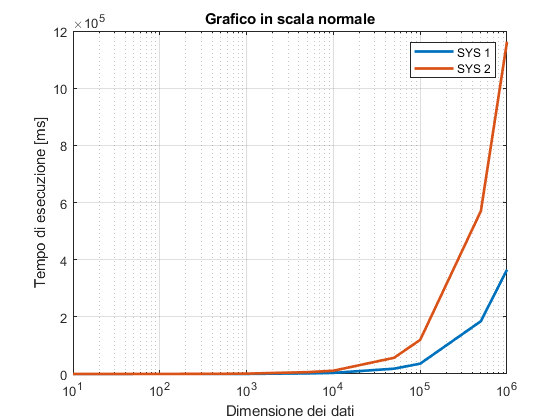
\includegraphics[width=0.8\textwidth]{img/hw0/grafico_naturale.png}
	\caption{\textit{Confronto andamento tempi di risposta sys1 e sys2}}
\end{figure}
\begin{figure}[H]
	\centering
	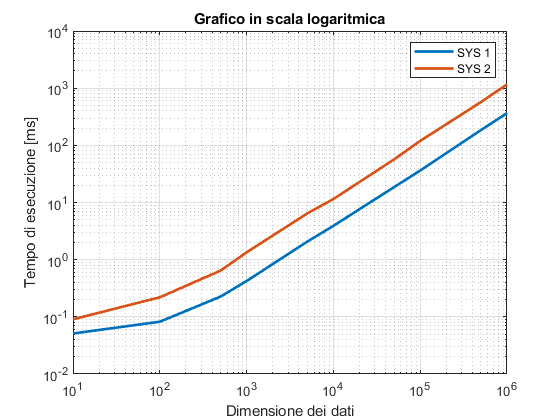
\includegraphics[width=0.8\textwidth]{img/hw0/grafico_log.png}
	\caption{\textit{Confronto andamento tempi di risposta - scala logaritmica}}
\end{figure}
Quindi il primo sistema è con evidenza quello più performante. Le differenze si percepiscono a vista d'occhio già a partire da \textit{N > $10^4$}.
\\Il motivo principale di tale differenza è proprio l'eterogeneità dei processori. Per quanto i due sistemi possano essere simili, il sistema più performante (Sistema 1) è dotato infatti non solo di un processore di architettura più avanzata, ma anche di alcune generazioni successive.